\documentclass[danish]{report}

\usepackage[utf8]{inputenc}
\usepackage[danish]{babel}
\usepackage{listings}
\usepackage{color}
\usepackage{courier}
\usepackage{parskip}

\definecolor{dkgreen}{rgb}{0,0.6,0}
\definecolor{gray}{rgb}{0.5,0.5,0.5}
\definecolor{mauve}{rgb}{0.58,0,0.82}

\lstset{
  frame=,
  language=C,
  aboveskip=3mm,
  belowskip=3mm,
  showstringspaces=false,
  columns=flexible,
  basicstyle={\small\ttfamily},
  numbers=none,
  numberstyle=\tiny\color{gray},
  keywordstyle=\color{blue},
  commentstyle=\color{dkgreen},
  stringstyle=\color{mauve},
  breaklines=true,
  breakatwhitespace=true
  tabsize=4
}

% clickable TOC
\usepackage{hyperref}
\hypersetup{
    colorlinks,
    citecolor=black,
    filecolor=black,
    linkcolor=black,
    urlcolor=black
}

\usepackage{graphicx}
\usepackage{hyperref}


% Title Page
\title{Obligatorisk opgave 1}
\author{Jacob B. Cholewa, Rasmus L. Wismann \& Nikolai Storr }


\begin{document}
\maketitle
\newpage
\tableofcontents
\newpage

\chapter{Introduktion}

I denne rapport vil vi beskrive hvordan vi har implementeret vores version af Shellen BOSC og den teori der ligger til grund for denne implementation. Rapporten er opdelt i tre sektioner, en introduktion, et implementations og teori afsnit og til sidste en konklusion. Næste sektion indeholder kravene til vores Shell.  

\section{Features}
\begin{enumerate}
\item bosh skal kunne virke uafhængigt. Du må ikke bruge andre eksisterende shells, f.eks. er det ikke tilladt at anvende et systemkald {\tt system()} til at starte {\tt bash}.
\item En bruger skal kunne indtaste almindelige enkeltstående kommandoer, så som {\tt ls}, {\tt cat} og {\tt wc}. Hvis kommandoen ikke findes i operativ systemet skal der udskrives en ”Command not found“ meddelelse.
\item Kommandoer skal kunne eksekvere som baggrundsprocesser (ved brug af \&) såadan at mange programmer kan køres på samme tid.
\item Der skal være indbygget funktionalitet som gør de muligt at lave redirection af stdin og stdout til filer. F.eks skal kommandoen {\tt wc -l < /etc/passwd > antalkontoer} lave en fil ”antalkontoer“, der indeholder antallet af brugerkontoer.
\item Det skal være muligt at anvende pipes. F.eks. skal {\tt ls | wc -w} udskrive antallet af filer.
\item Funktionen {\tt exit} skal være indbygget til at afslutte shell’en.
\item Tryk på Ctrl-C skal afslutte det program, der kører i {\tt bosh} shell’en, men ikke shell’en selv.
\end{enumerate}

\chapter{Implementation og teori}
\section{Feature 1 og 2}
Første krav til vores shell er at vi ikke bruger andre shells til at få vores shell eller systemkald til at virke. Det skal altså være et selvstående program. En shell er en grafisk brugergrænseflade der tillader brugeren at inputte og køre programmer. Shellen er altså en process der kan starte andre programmer som processer. For at en bruger kan eksekvere programmer på maskinen så som {\tt ls}, {\tt cat} og {\tt wc} skal vi kigge i de forskelle {\tt bin} arkiver. Vi har skrevet vores shell til linux systemer, og vi leder derfor efter det inputtede program i mapperne {\tt ./}, {\tt /bin/} og {\tt /usr/bin/}. Hvis vi finder programmet som brugeren prøver at starte bruger vi vi det indbyggede program i linux {\tt execvp}. {\tt execvp} programmet tager en process og bytter det ud med en anden process. Det første vi gør er derfor at oprette en nye process med {\tt fork()}. Fork opretter en kopi af den eksisterende process. Den nye process kaldes for en \textit{child process} og den eksisternede process for en \textit{parrent process}. Dette gøres med følgende kode.

\begin{lstlisting}

... Parrent process code

pid_t pid = fork();
if(pid == 0){
    ... Child process code ...
}else{
    ... Parrent process code ...
}

... Parrent and child process code ...

\end{lstlisting}

Når vi har lavet et kopi af shell processen bytter vi ved brug af {\tt execvp} \textit{child processen} ud med det program som brugeren ønskede at starte. På den måde kan vi starte programmer som nye processer fra vores BOSC shell.

\section{Feature 3}
\section{Baggrundsproces}

Hvis en kommando køres med symbolet {\tt \&} skal processen startes som en baggrundsprocess. Vi ønsker denne feature fordi at en bruger skal kunne køre flere programmer fra shell'en på samme tid. Når vi starter en process vil vi gerne vente på den terminiene inden vi igen tillader input fra brugeren. Dette gør vi med {\tt waitpid(process\_id, status\_location, options)}. Når vi starter en baggrundsproces vælger altså derfor blot ikke at vente på barne processen og lader derfor strakts brugeren indtaste nyt input. Som det kan ses i kode stykket nedenfor venter vi derfor kun på barne processen hvis {\tt background} er {\tt 0} ({\tt false}). {\tt shellcmd} er en struct vi bruger til at holde brugerens kommando. 
\begin{lstlisting}
int executeshellcmd(Shellcmd *shellcmd){
    

    ... code to check shellcmd

    pid_t pid = fork();
    if(pid == 0){
           ... Code executing the user input program ...
    }else{
        if(shellcmd -> background == 0){
            int wstatus = 0;    
            waitpid(pid,&wstatus,0);
        }
    }
    return 0;
}
\end{lstlisting}

\section{Redirect}
\label{redirect}
I Linux bliver input devices og data streams betragtet som filer. En file descriptor er et handle til en åben fil.

En file descriptor er et index i en tabel. Hver process har en file descriptor tabel. Tabellen indeholder descriptors der giver processen adgang til åbnede filer, sockets, pipes og kernel-level strukturer.   

En bash shell har automatisk adgang til tre file descriptors, StdIn, StdOut og StdErr. StdIn, StdOut og StdErr er alle character devices i linux. De sender en strøm af bytes fra shell'en til en underliggende process.  

StdOut  beskrives med file descriptor 1. StdIn beskrives med file descriptor 0. Når outputttet fra én proces' file descriptor 1 sendes til inputtet fra en anden proces' file descriptor 0, redirectes brugerens input fra den første process til den anden. Samtidig lukkes de ubrugte input og output.   

Linux har to redirection operators, {\tt >} og {\tt <}, som begge gør netop dette. Et system kald, {\tt p1 > p2}, fungerer ved at p2's input file descriptor sættes til p1's output file descriptor. Systemet lukker samtidig p2's gamle input filedescriptor samt p1's gamle output file descriptor. 

I system kaldet  {\tt p1 < p2} sættes p1's input file descriptor til p2's output file descriptor. Systemet lukker også p1's gamle input filedescriptor samt p2's gamle output file descriptor. 

Denne modulare fremgangsmåde gør at man i Linux kan bygge stadig større funktionalitet op ved at sammensætte system kald.  
   
\subsection{Implementation}
Hvis symbolet {\tt >} optræder i kommandoen skal vi ifølge opgaven omdirigere output til filnavnet på venstre side. eg. {\tt cmd > file}. På samme måde skal vi hvis symbolet {\tt <} optræder i kommandoen omdirigere input til at være filen fra venstre side. eg {\tt cmd < file}. 

Dette har vi implementeret med følgende logik.

\begin{lstlisting}
if(in == NULL && out == NULL){
                status = executecmd(cmdlist);
            }else{
                if(in != NULL && out != NULL) status = redirInOut(in, out, cmdlist);
                if(in != NULL) status = redirIn(in, cmdlist);
                if(out != NULL) status = redirOut(out, cmdlist);
            }
\end{lstlisting}

som bruger følgende hjælpe metoder.

\begin{lstlisting}
// redirect in and out
int redirInOut(char *inFile, char *outFile, Cmd *cmdlist){
    
    int fidIn  = open(inFile, O_RDONLY);
    int fidOut = open(outFile, O_WRONLY | O_CREAT | O_APPEND);              
    close(0); close(1);
    dup(fidIn); dup(fidOut);
    int status = executecmd(cmdlist);
    close(fidIn); close(fidOut);
    if(status != 0) 
        printf("execvp returned: %i, errno returned: %i 'no such file or directory' \n", status, errno);

}

// redirect in
int redirIn(char *inFile, Cmd *cmdlist){
    int fid = open(inFile, O_RDONLY);  
    close(0); // close standard input
    dup(fid);   // 'duplicate fileid', opens another input (file)    
    int status = executecmd(cmdlist);
    close(fid);             
    if(status != 0) 
        printf("execvp returned: %i, errno returned: %i 'no such file or directory' \n", status, errno);


}

// redirect out
int redirOut(char *outFile, Cmd *cmdlist){
    int fid = open(outFile, O_WRONLY | O_CREAT | O_APPEND);         
    close(1); // close standard output
    dup(fid); // duplicate file-descriptor

    int status = executecmd(cmdlist);
    close(fid);             
    if(status != 0) 
        printf("execvp returned: %i, errno returned: %i 'no such file or directory' \n", status, errno);

}
\end{lstlisting}


De tre redirect metoder bruger alle samme logik. 

Vi åbner den fil som optræder i shell input kommandoen (husk, alle I/O objekter (streams, devices) betragtes som filer i Linux ).  {\tt open} kommandoen returnerer altså en file descriptor. 

Dernæst lukkes de gamle StdIn og StdOut hvorefter vi duplikerer den åbne fil descriptor med {\tt dup} system kaldet. 

Nu eksekveres så resten af command listen (executecmd(cmdlist)) i.e., andre processer forkes som nu arver de input output vi har sat op i vores redirect. Til sidst lukkes filen/filerne  igen. 

Sammen med {\tt pipe} bruges {\tt dup} i Linux til at konstruere pipes mellem processers standard input og ouput (se \ref{pipe}).


\section{Pipe}
\label{pipe}
% ??? 
%En pipe (c1 {\tt | c2}) tager outputtet fra kommandoen på %højre side og bruger det som input til kommandoen på %venstre side. E.g. {\tt c1 | c2 | c3 } tager output fra c1 %og giver til c2 som input osv. 


Pipes er en form for inter-process-communication (IPC) i Linux. En pipe associerer outputtet fra én process med en in-memory buffer i systemet. Andre processer kan nu associere deres input med denne buffer og derefter forbruge outputtet fra processen. 

Et {\tt pipe(fd)} kald tager et enkelt argument, {\tt fd[2]}, en array med to elementer. De to elementer repræsenterer file descriptors for et input og et output. pipes bruges typisk mellem en parent og child process. Først oprettes et argument arrray, dernæst etableres en {\tt pipe(fd)}. Derefter forker man processen hvilket medfører at alt data fra forældreren kopieres, inklusive pipen. 

Hvis forældreren ønsker at modtage data fra barnet lukkes forældrens {\tt fd[1] }, og barnets {\tt fd[0]}. Hvis det modsatte er tilfældet bytter man  rundt på disse. Siden file descriptors er delt mellem forældre og barne process skal man huske også, at lukke den ubrugte ende af pipen.


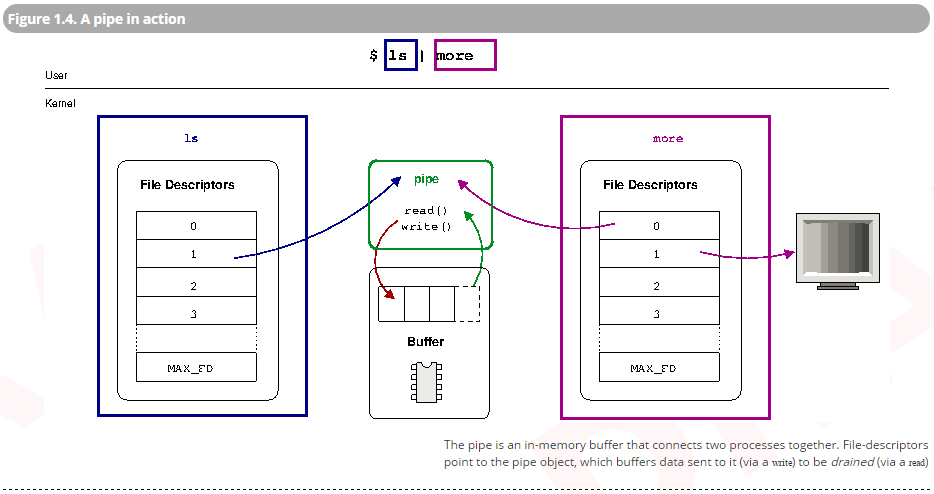
\includegraphics[scale=0.5]{pipe}

Hvis pipe bufferen er tom vil den modtagende process blokere indtil der er data tilgængelig. Dette kan i sig selv bruges som kommunikationsstrategi. Alt hvad den skabende process behøver for at signalere den modtagende process, er at sende en enkelt byte.

\subsection{dup}
Ofte kan barne processens standard in og output file descriptors duplikeres ved hjælp af system kaldet {\tt dup} . Efter system kaldet {\tt dup} kan barneprocessen eksekvere helt tredje processer som så vil arve standard input og standard output fra barnet. 

{\tt dup} system kaldet bruger altid den kaldende proces' lavest nummererede ubrugte file descriptor (dvs. lukkede descriptor), i.e., hvis {\tt fd[1]} er tilgængelig , bruges denne.

Dette betyder at man typisk starter i barneprocessen af en pipe. Først lukkes den file descriptor man ikke skal bruge, og dernæst kaldes {\tt dup} som så duplikerer den ubrugte file descriptor over som en af de de nye standard input  output file descriptors. De processer der herefter eksekveres fra barneprocessen arver nu disse input og output som deres StdIn og StdOut.


\subsection{Implementation}
Vi har i vores shell implementeret pipes ved hjælp af følgende logik. {\tt executecmd} metoden kaldes af de metoder som er vist i \ref{redirect}.

Først opretter vi en {\tt pipe} med en {\tt int fd[2]} array som argument og så forker vi en ny process. Dernæst lukker vi dennes input samt forældreprocessens ouput. Så sætter vi {\tt fd} arrayens to elementer til processernes respektive filedescriptors med {\tt dup}. Til sidst kalder vi rekursivt metoden igen indtil der ikke er flere commands i {\tt cmdlist }. 

På den måde piper vi inputtet fra én command ind i den næste, og så fremdeles, ned gennem en liste  af commands. 


\begin{lstlisting}
int executecmd(Cmd *cmdlist){
    int status;
    char **cmd = cmdlist -> cmd;
    Cmd *next = cmdlist -> next;
    if(next != NULL){

        int fd[2];
        pipe(fd);

        pid_t pid = fork();
        if(pid == 0){
            close(fd[0]);
            close(1);
            dup(fd[1]);
            close(fd[1]);
            status = executecmd(next);
        }else{
            close(fd[1]);
            close(0);
            dup(fd[0]);
            close(fd[0]);
            status = execvp(*cmd,cmd);
            
            int wstatus;
            waitpid(pid,&wstatus,0);
        }
    }else{
        status = execvp(*cmd,cmd);
    }
    return status;
}

\end{lstlisting}

\section{Exit}

%Denne funktion er allerede forklaret som en del af feature 6. 

I 'executeshellcmd' samler vi alle commands og sender dem til funktionen 'isValidCmd' for validering (unødvendigt, da execute funktionerne allerede returnerer -1 hvis en command ikke findes). Som sagt under Feature 2 returnerer denne funktion -1 Hvis 'exit' er en command. 'executeShellCmd' returnerer så umiddelbart 1 til 'main' metoden. Dermed terminerer while loopet i 'main' og vores shell slutter. 

I executeShellCmd() samler vi alle commands og sender dem til validering. Hvis status er -1 returnerer vi fra funktionen.


\begin{lstlisting}
while( cmdlist != NULL){
	char **cmd = cmdlist -> cmd;
	cmdlist = cmdlist -> next;
	status = isValidCmd(cmd);

	if(status == 0){ 
		printf("%s: command not found\n", *cmd );
		return 0;
	}
	if(status == -1) return 1;
}
\end{lstlisting}

I isValidCmd() returnerer vi -1 hvis 'exit' er en command.
\begin{lstlisting}
int isValidCmd(char **cmd){
	
	if(strncmp(*cmd,"exit",4) == 0) return -1;
\end{lstlisting}

I main(). Terminering af while loopet afslutter vores shell. 
\begin{lstlisting}
/* parse commands until 'exit' command, then exit */
while (!terminate) {
	terminate = executeshellcmd(&shellcmd);
\end{lstlisting}

\section{Ctrl-c}

Et signal eller et interrupt er en event som midlertidigt overlader program kontrollen til et andet program eller funktion. Når funktionen eller programmet er færdigt kan kontrollen overlades til den 'interruptede' process som så kan fortsætte. Man skelner mellem hardware og software interrupts.

Et software interrupt eller signal er en asynkron aktivitet. i.e., processer venter ikke på signalet. Det program eller den funktion der er designet til at svare på en event siges at fange den, eller på engelsk,  at 'trap' eller 'handle' eventen. Derfor kaldes den typisk en 'signal handler'. 

Et program tildeles en række default handlers som udgør events som det kan 'fange'. For eksempel, hvis et program kører i en prompt vil tastekombinationen ctrl-c blive fanget af en handler, hvis default handling er, at terminere processen. 

\subsection{Implementation}
Vi har implementeret en signal handler der fanger ctrl-c interrupts. Hver gang vi forker en ny process attacher vi vores signal handler. Det sker både i executecmd metoden og i executeshellcmd metoden fordi vi forker nye processer begge disse to steder. 

\begin{lstlisting}
...
pid_t pid = fork();
if(pid == 0){
	// setup a signal handler for this thread
	signal(SIGINT, leave);
...
\end{lstlisting}

Når man herefter trykker ctrl-c bliver program kontrollen overført til vores handler metode. Her kan vi så exitte processen hvis det er en child process. Hvis det ikke er , må det være vores bosh shell selv, og så gør metoden intet. 

\begin{lstlisting}
// signal handler
void leave(int sig){
	pid_t pid = getpid();
	if(pid == 0){
		// thread interrupt
		exit(sig);
	}
}
\end{lstlisting}

Herefter gives kontrollen tilbage til vores bosh shell.

\chapter{Konklusion}
\end{document}          
